\section{M2 multiband alignment and gauge-resolved locality}
\label{app:supp-m2}

\subsection{Identity and evidence boundary}

M2 is the prospectively frozen local synthetic calculation with identity
\begin{center}
 \small\path{icmsep2026.paper1.periodic1d.}\\
 \path{multiband-alignment.v1}
\end{center}
Its retained package is
\begin{center}
 \small\path{calculations/ICMSEP2026/conference/paper_1/}\\
 \path{multiband-alignment/}.
\end{center}
The producer composes maintained frame transport, pointwise alignment,
operator projection, Fourier transformation, block-hopping truncation,
interpolation, and band-error Actions. The retained verifier reconstructs the
finite protocol without calling the producer Action.

M2 establishes bounded numerical behavior for one constructed rank-two
example. It does not establish material validity, uncertainty bounds,
continuum convergence, a general nonconvex alignment solver, or scientific
acceptance. In particular, the exact pointwise Procrustes channel is kept
separate from the constrained family containing one global unitary over the
whole reciprocal path.

\subsection{Gapped parent and frozen sampling}

The four-state parent is the block polynomial
\begin{equation}
 H(k)=T_0+e^{2\pi i k}T_1+e^{-2\pi i k}T_1^\dagger,
 \qquad k\in[-1/2,1/2),
 \label{eq:supp-m2-parent}
\end{equation}
with
\begin{equation}
 T_0=\begin{pmatrix}
 -1.20&0.06&0&0\\0.06&-0.35&0&0\\
 0&0&1.00&0.04\\0&0&0.04&1.75
 \end{pmatrix},\quad
 T_1=\begin{pmatrix}
 0.15&0&0&0\\0&-0.10&0&0\\
 0.12&0&0.05&0\\0&0.10&0&-0.04
 \end{pmatrix}.
 \label{eq:supp-m2-blocks}
\end{equation}
The two lowest eigenstates define the retained composite space. The training
mesh has 64 centered half-open points. The 257 withheld points use the frozen
staggered rule recorded in the result and are disjoint from training. The
observed minimum separation between the retained group and the upper group is
$1.0566461211497047$, above the frozen lower bound $0.5$. The minimum singular
value among neighboring and closure overlaps is
$0.9999828868735376$, above the frozen transport threshold $0.8$.

\subsection{Sewing, transport, and known gauge attack}

Raw retained eigenframes are polar transported along the ordered mesh and
closed using identity reciprocal-boundary sewing. For transported frame
$U(k)$, the known periodic attack is
\begin{equation}
 \widetilde U(k)=U(k)A(k),\qquad
 A(k)=\begin{pmatrix}\cos\theta(k)&-\sin\theta(k)\\
 \sin\theta(k)&\cos\theta(k)\end{pmatrix},
 \label{eq:supp-m2-attack}
\end{equation}
where
\begin{equation}
 \theta(k)=0.30+0.65\sin(2\pi k)+0.30\sin(4\pi k).
 \label{eq:supp-m2-angle}
\end{equation}
The projector defect between $U$ and $\widetilde U$ is
$3.24\times10^{-16}$, while their maximum frame defect is $1.506$.
Thus the retained state space is unchanged although its matrix frame changes.
The closure eigenphases are $0.01416$ and $0.01878$ radians; they are retained
as finite-mesh transport diagnostics, not as a topological classification.

At each point, Procrustes alignment recovers $A(k)^\dagger$ with maximum
rotation defect $6.77\times10^{-16}$. The aligned-frame defect is
$7.00\times10^{-16}$. By contrast, the separately frozen constrained family
uses one global unitary $C$ for all points. Its optimum for the sampled path is
numerically the constant rotation by $-0.30$ radians, and its maximum frame
defect remains $1.131$. This comparison diagnoses the limitation of that
specific constrained family; it is not a failed global search over arbitrary
smooth gauges.

\subsection{Projected operators and complete block hoppings}

For each frame $V(k)$, the represented retained operator is
\begin{equation}
 H_V(k)=V(k)^\dagger H(k)V(k).
 \label{eq:supp-m2-projected}
\end{equation}
The attacked representation differs from the transported representation by a
maximum Frobenius defect $0.9972$, although their unordered spectra are
identical. Pointwise alignment reduces this matrix defect to
$9.83\times10^{-16}$. The one-global-unitary channel leaves a maximum defect
$0.7443$. These are frame-dependent matrix diagnostics after explicit
identification; the common projector and spectra are invariant channels.

Complete 64-point Fourier transforms reconstruct the transported, attacked,
and pointwise-aligned matrix samples with maximum Frobenius errors
$6.76\times10^{-16}$, $1.14\times10^{-15}$, and
$6.77\times10^{-16}$, respectively. Their block-Hermiticity defects are at
most $4.50\times10^{-17}$. Complete reconstruction verifies the finite
discrete transform; it does not establish unsampled continuum interpolation.

\begin{figure}[t]
 \centering
 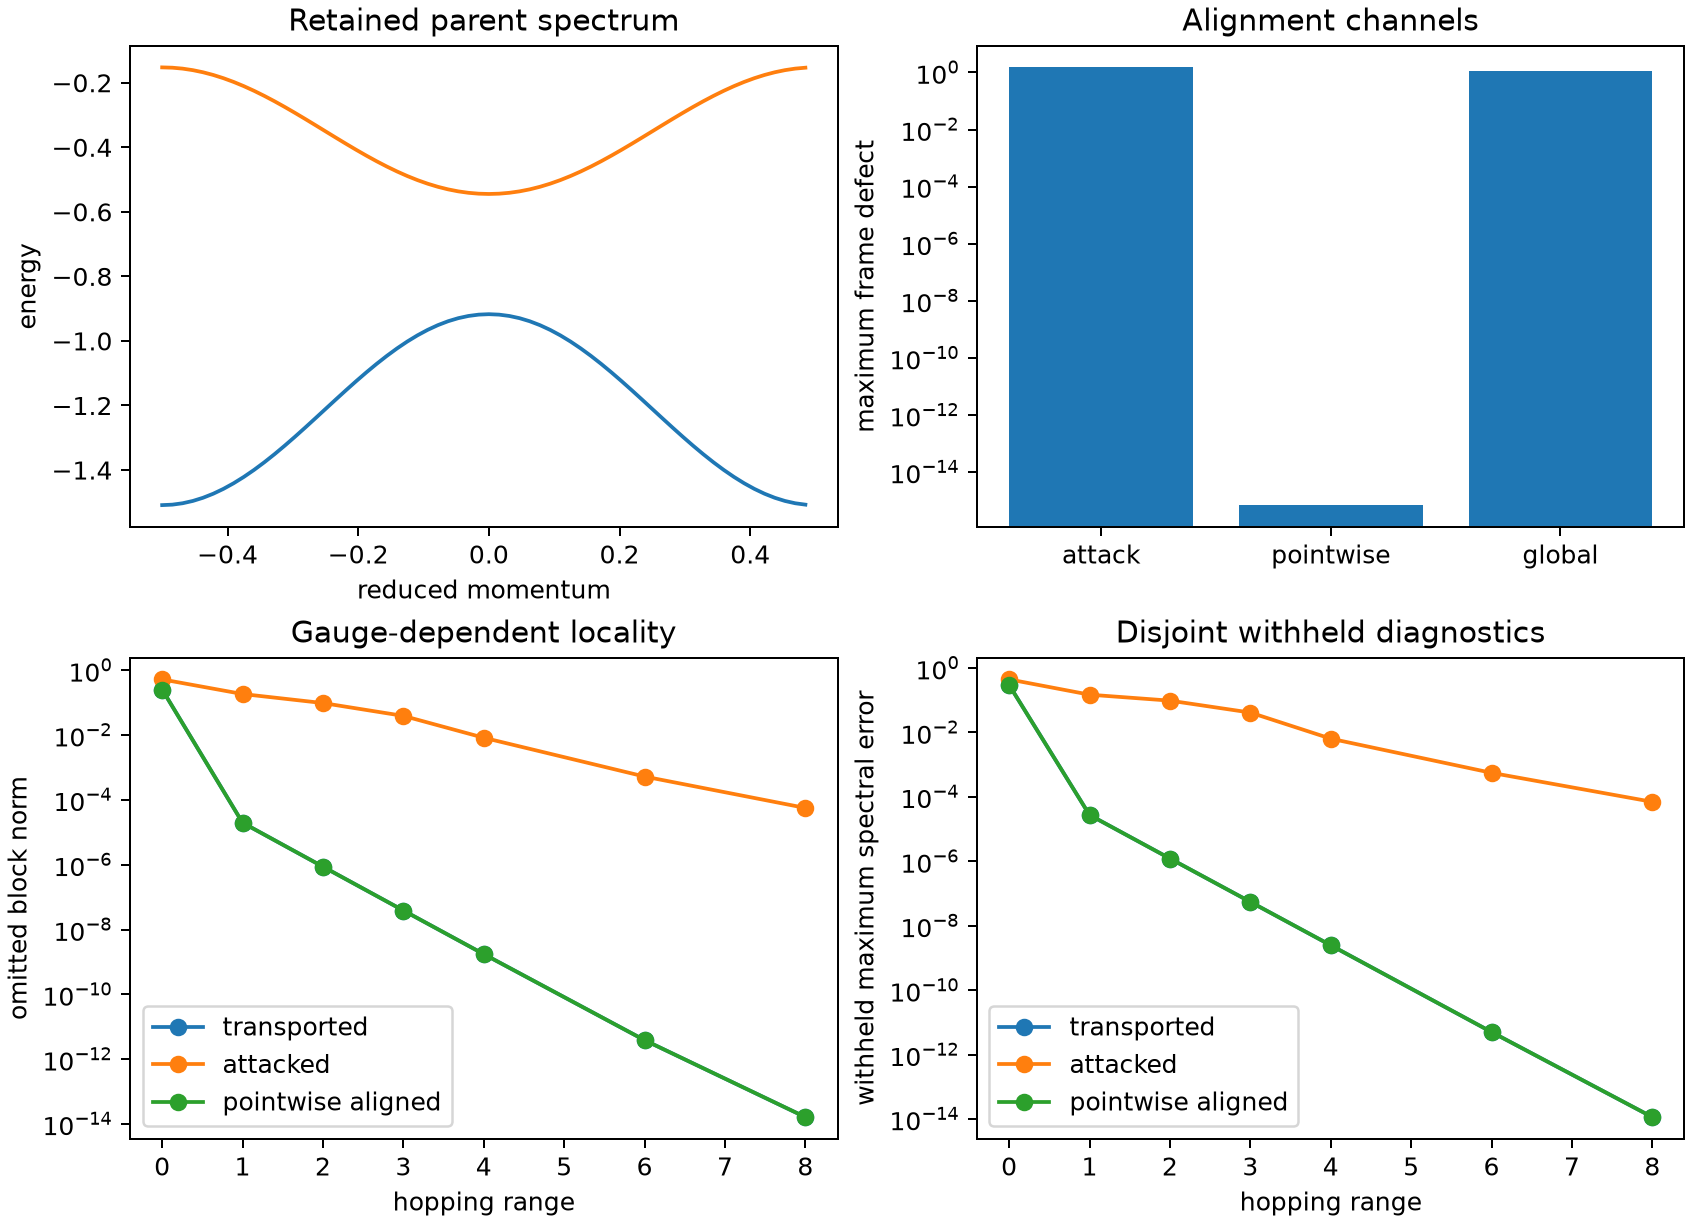
\includegraphics[width=0.97\linewidth]{../../../../../calculations/ICMSEP2026/conference/paper_1/multiband-alignment/multiband-alignment-summary.png}
 \caption{Frozen M2 retained spectrum, alignment channels, omitted block norms,
 and disjoint withheld maximum spectral errors. The exact pointwise channel is
 distinct from the one-global-unitary constrained family.}
 \label{fig:supp-m2-summary}
\end{figure}

\subsection{Gauge-resolved truncation and withheld checks}

Symmetric truncations retain representatives $|R|\leq R_{\max}$. Table
\ref{tab:supp-m2-ranges} reports selected values from the frozen range
sequence. The transported and pointwise-aligned frames recover the same local
behavior to floating-point error. In the attacked frame,
\[
 \widetilde H(k)=A(k)^\dagger H(k)A(k).
\]
Writing $H(k)=\sum_R e^{2\pi i kR}T_R$ and
$A(k)=\sum_m e^{2\pi i km}A_m$ gives the Fourier convolution
\[
 \widetilde T_Q=\sum_{m,n}A_m^\dagger T_{Q+m-n}A_n.
\]
A momentum-dependent unitary therefore mixes hopping coefficients across
ranges even though it preserves each fiber spectrum and retained projector; a
constant unitary has only its zero Fourier mode and merely conjugates each
block. Thus spectral and projector agreement do not protect finite-range
tight-binding locality or compressibility. The periodic attack redistributes
the same spectral information into a longer block-hopping tail. At range eight,
its omitted-block norm is $5.65\times10^{-5}$ and its withheld maximum spectral
error is $7.04\times10^{-5}$, compared with approximately
$1.6\times10^{-14}$ and $1.2\times10^{-14}$ for the transported channel.

\begin{table}[t]
\centering
\scriptsize
\caption{Selected M2 omitted-block norms and withheld maximum spectral errors.}
\label{tab:supp-m2-ranges}
\begin{tabular}{@{}rrrrrr@{}}
\toprule
$R_{\max}$ & $\|T\|_{\mathrm{omit}}$ & $\|\widetilde T\|_{\mathrm{omit}}$
& transported error & attacked error & aligned error\\
\midrule
0 & $2.54\!\times\!10^{-1}$ & $5.23\!\times\!10^{-1}$
  & $2.98\!\times\!10^{-1}$ & $4.45\!\times\!10^{-1}$ & $2.98\!\times\!10^{-1}$\\
1 & $1.98\!\times\!10^{-5}$ & $1.85\!\times\!10^{-1}$
  & $2.76\!\times\!10^{-5}$ & $1.49\!\times\!10^{-1}$ & $2.76\!\times\!10^{-5}$\\
4 & $1.75\!\times\!10^{-9}$ & $8.28\!\times\!10^{-3}$
  & $2.49\!\times\!10^{-9}$ & $6.43\!\times\!10^{-3}$ & $2.49\!\times\!10^{-9}$\\
8 & $1.63\!\times\!10^{-14}$ & $5.65\!\times\!10^{-5}$
  & $1.15\!\times\!10^{-14}$ & $7.04\!\times\!10^{-5}$ & $1.15\!\times\!10^{-14}$\\
\bottomrule
\end{tabular}
\end{table}

Withheld values evaluate only already fixed finite-range models. They do not
alter the parent, frame transport, attack, alignment family, hopping ranges,
thresholds, or figure-data selection.

\subsection{Independent verification and provenance}

The retained verifier independently rebuilds the parent polynomial,
eigenspaces, polar transport, periodic attack, pointwise and global
alignments, projected operators, Fourier blocks, Hermiticity defects,
truncations, omitted norms, and training/withheld spectral errors. Its maximum
dimensionless defect is $1.33\times10^{-15}$ and its maximum energy-channel
defect is $7.43\times10^{-15}$, both below the frozen $10^{-11}$ tolerance.

The input and protocol were hashed before the confirmatory calculation. The
package retains the protocol freeze, result, independent verification,
figure-data CSV, figure, report, software environment, source manifest, and
artifact checksums. The software record reports Python 3.14.6, NumPy 2.5.1,
SciPy 1.18.0, Matplotlib 3.11.1, and \texttt{ksdft2effmass 0.1.0.dev0}; the
dirty worktree is bound by \texttt{source.sha256}. No external calculator was
invoked.
